%!TEX root = ../principal.tex
\setchapterimage[7.5cm]{figs/aproximados/domo}
\setchapterpreamble[u]{\margintoc}

\chapter{Métodos aproximados} \label{chap:aproximados}

\begin{kaobox}
	``Calidad significa hacerlo bien cuando nadie está mirando"
	
	``Una de las grandes sorpresas del hombre es encontrar que puede hacer lo que temía no podía hacer"
	\begin{flushright}
		Henry Ford
	\end{flushright}
\end{kaobox}

La incógnita maestra es el campo de desplazamientos $\mathbf{u}$, los métodos aproximados, en general, se basan en suponer un campo de desplazamientos $\tilde{\mathbf{u}}$ y aplicar algunos criterios para aproximarlo a la solución exacta $\mathbf{u}$ lo mejor posible.

\section{Método de Rayleigh-Ritz}

En el presente método se realiza la construcción del campo de desplazamientos $\tilde{\mathbf{u}} = \begin{bmatrix}
	\tilde{u} & \tilde{v} & \tilde{w}
\end{bmatrix}^T$ como combinación lineal de ciertas funciones:

\marginnote[2cm]{$n > m > l$}
\begin{equation}
	\begin{split}
		\tilde{u}(x, y, z) = \sum_i a_i \phi_i(x, y, z) & \qquad \forall \ i = 0, \dots, l-1\\
		\tilde{v}(x, y, z) = \sum_j a_j \phi_j(x, y, z) & \qquad \forall \ j = l, \dots, m - 1 \\
		\tilde{w}(x, y, z) = \sum_k a_k \phi_k(x, y, z) & \qquad \forall \ k = m, \dots, n - 1
	\end{split}
\end{equation}

Las $n$ funciones $\phi_i(x, y, z)$ usualmente son polinomios. Los desplazamientos $\tilde{\mathbf{u}}$ necesitan satisfacer \textit{solo las condiciones esenciales} de frontera.
\marginnote[]{Las funciones de aproximación deben satisfacer solo las condiciones esenciales de frontera}

Con estas funciones aproximadas la energía potencial \eqref{eq:EP} se convierte en:

\begin{equation}
	\Pi = \Pi(a_0, a_1, \dots a_{r-1})
\end{equation}

En donde $r$ es el número de incógnitas independientes.

De acuerdo al principio de mínima energía potencial, se debe cumplir:

\begin{equation}
	\dfrac{\partial \Pi}{\partial a_i} = 0 \qquad \forall \; i = 0, \dots, r - 1
\end{equation}

\begin{example}
	Calcule el campo de desplazamientos para la barra de la fig. \ref{fig:BarraVertical}, utilizando el método de Rayleigh-Ritz. Datos de la barra: densidad $\rho$, módulo de elasticidad $E$, sección transversal $A$, longitud $L$.
	
	
	\begin{marginfigure}[-1cm]
		\centering
		\includestandalone[width=.4\textwidth]{figs/aproximados/barra0}
		\caption{Barra vertical bajo acción de la gravedad.}
		\label{fig:BarraVertical}
	\end{marginfigure}
	
	\textit{Solución}:
	\vspace{2mm}
	
	Se supone:
	\begin{equation}
		u(x) = a_0 + a_1 x + a_2 x^2
	\end{equation}
	que debe cumplir las condiciones esenciales de frontera:
	
	\begin{equation}
		\begin{cases}
			u(0) = 0 \implies a_0 = 0 \\
			u(L) = 0 \implies a_2 = -\dfrac{a_1}{L}
		\end{cases}
	\end{equation}
	
	entonces:
	\begin{equation}
		u(x) = a_1 x \left(1 - \dfrac{x}{L}\right)
		\label{eq:rr1}
	\end{equation}
	
	cuya derivada es:
	\begin{equation}
		\dfrac{du}{dx} = a_1 \left( 1 - \dfrac{2}{L}x \right)
		\label{eq:der1}
	\end{equation}
	
	Según \eqref{eq:eptuni}, la energía potencial total es:
	\begin{equation*}
		\Pi = \dfrac{1}{2} \int_L EA \left( \dfrac{du}{dx} \right)^2 \, dx - \int_L up\, dx - \sum_i u_i P_i
	\end{equation*}
	
	en este caso, la carga por unidad de longitud $p = A \rho g$ y no existen cargas puntuales, es decir: $P_i = 0$.
	
	Substituyendo \eqref{eq:der1} en la expresión de la energía potencial y haciendo,
	\begin{equation*}
		\dfrac{\partial \Pi}{\partial a_1} = 0 
	\end{equation*}
	
	
	se obtiene el resultado deseado:
	\begin{equation}
		u(x) = \dfrac{\rho g L}{2E} x \left(1 - \dfrac{x}{L}\right)
		\label{eq:rr2}
	\end{equation}
\end{example}

\section{Método de residuos ponderados}

Básicamente son métodos para resolver ecuaciones diferenciales.

La idea parte de recordar que, en un sistema de ecuaciones lineales $\mathbf{Ax} = \mathbf{b}$, si $\mathbf{b} \not \in C(\mathbf{A})$, siendo $\mathbf{p}$ el vector proyección de $\mathbf{b}$ sobre el espacio columna $C(\mathbf{A})$, el vector error o \textit{residuo} $\bm{\epsilon} = \mathbf{b} - \mathbf{p}$ es ortogonal a $C(\mathbf{A})$ y por lo tanto pertenece al espacio nulo izquierdo, es decir $\bm{\epsilon} \in N(\mathbf{A}^T)$, ya que $C(\mathbf{A})^{\perp} = N(\mathbf{A}^T)$, entonces:
\begin{equation}
	\mathbf{A}^T \mathbf{y} = \mathbf{0}
	\label{eq:residuo}
\end{equation}

Se extienden estas ideas al espacio de Hilbert\sidenote{David Hilbert, alemán (23 Enero 1862 – 14 Febrero 1943)}. Suponga $\mathbf{y} \rightarrow \bm{\epsilon}$ y que la ecuación diferencial del problema sea:
\begin{equation}
	L \mathbf{u} = \mathbf{P}
	\label{eq:LuP}
\end{equation}
En donde $L$ es un operador diferencial y $\mathbf{P}$ una función vectorial.

Si se aproxima el campo vectorial $\mathbf{u}$ con $\tilde{\mathbf{u}}$, la solución ya no es exacta, habrá un residuo, el cual será:
\begin{equation}
	\bm{\epsilon} = L \tilde{\mathbf{u}} - \mathbf{P}
\end{equation}

Las funciones de aproximación $\tilde{\mathbf{u}}$ deben cumplir con \textit{todas} las condiciones de frontera, esenciales y naturales.\marginnote[]{Las funciones aproximadoras, en los métodos de residuos ponderados, deben cumplir con todas las condiciones de frontera.}

Entonces \eqref{eq:residuo} se convierte en:
\begin{equation}
	\int_V \mathbf{w}^T \bm{\varepsilon} \, dV = 0
	\label{eq:pond}
\end{equation}

La elección de $\mathbf{w}$ lleva a diferentes métodos de resolución, un par de ellos son el método de mínimos cuadrados y el de Galerkin\sidenote{Boris Grigoryevich Galerkin, ruso (4 Marzo 1871 – 12 Julio 1945)}.

\subsection{Mínimos cuadrados}
Se trata de minimizar la suma de los cuadrados de los errores, en este contexto la expresión matemática es:
\begin{equation}
	\min S: \quad S = \int_V ||\bm{\varepsilon}||^2 \, dV =  \int_V \bm{\epsilon}^T \bm{\epsilon} \, dV
\end{equation}

si $\tilde{\mathbf{u}}$ depende de parámetros $a_i$, entonces:
\begin{equation}
	\dfrac{\partial S}{\partial a_i} = 2 \int_V \bm{\epsilon}^T \dfrac{\partial \bm{\epsilon}}{\partial a_i} \, dV = 0
\end{equation}

es decir, las funciones ponderadoras son las derivadas del residual:
\begin{equation}
	\boxed{\int_V \bm{\epsilon}^T \dfrac{\partial \bm{\epsilon}}{\partial a_i} \, dV = 0}
\end{equation}

Para casos unidimensionales en barras de sección constante:
\begin{equation}
	\int_L \epsilon \dfrac{\partial \epsilon}{\partial a_i} \, dx = 0
	\label{eq:min2}
\end{equation}

\begin{exercise}
	Calcule el campo de desplazamientos para la barra de la \reffig{BarraVertical}, utilizando el método de los mínimos cuadrados. Datos de la barra: densidad $\rho$, módulo de elasticidad $E$, sección transversal $A$, longitud $L$.
	
	\begin{marginfigure}[-.5cm]
		\centering
		\includestandalone[width=.4\textwidth]{figs/aproximados/barra0}
		\repeatcaption{fig:BarraVertical}{Barra Vertical.}
	\end{marginfigure}
	
	
\textit{Solución}:

\vspace{2mm}
		Se supone:
		\begin{equation}
			u(x) = a_0 + a_1 x + a_2 x^2
		\end{equation}
		que debe cumplir con todas las condiciones de frontera, las esenciales y las naturales, en este caso solo se tienen las esenciales.
		
		\begin{equation}
			\begin{cases}
				u(0) = 0 \implies a_0 = 0 \\
				u(L) = 0 \implies a_2 = -\dfrac{a_1}{L}
			\end{cases}
		\end{equation}
		
		entonces:
		\begin{equation}
			u(x) = a_1 x \left(1 - \dfrac{x}{L}\right)
			\label{eq:min1}
		\end{equation}
		
		La ecuación de campo es:
		
		\begin{equation}
			\dfrac{d}{dx} \left(EA \dfrac{du}{dx}\right) + p = 0
		\end{equation}
		
		La carga por unidad de longitud es: $p = A \rho g$, la ec. de campo es por tanto:
		
		\begin{equation}
			\dfrac{d^2 u}{dx^2} + \dfrac{\rho g}{E} = 0
		\end{equation}
		
		observando \eqref{eq:min1} se tiene: $\dfrac{d^2 u}{dx^2} = -\dfrac{2a_1}{L}$, por tanto el residual es:
		
		\begin{equation}
			\epsilon = -\dfrac{2a_1}{L} + \dfrac{\rho g}{E}
		\end{equation}
		
		su derivada respecto a $a_1$ es:
		
		\begin{equation}
			\dfrac{\partial \epsilon}{\partial a_1} = -\dfrac{2}{L}
		\end{equation}
		
		aplicando \eqref{eq:min2} se tiene:
		
		\begin{equation}
			\int_{0}^{L} \dfrac{2}{L} \left( \dfrac{2a_1}{L} - \dfrac{\rho g}{E} \right) \, dx = 0
		\end{equation}
		
		de donde: $a_1 = \dfrac{\rho g L}{2E}$, así finalmente:
		
		\begin{equation}
			u(x) = \dfrac{\rho g L}{2E} x \left(1 - \dfrac{x}{L}\right)
		\end{equation}
		
		que es idéntico a \eqref{eq:rr2}.
\end{exercise}

\subsection{Método de Galerkin}

Observe que \eqref{eq:pond}, básicamente, implica \textit{igualar a cero la ecuación diferencial, multiplicarla por funciones ponderadoras e integrar}.

En el método de Galerkin, para el sistema de ecuaciones \eqref{eq:LuP}, se admite una función aproximadora de la forma:

\begin{equation}
	\tilde{u} = \sum_i a_i \phi_i
	\label{eq:gal1}
\end{equation}
\marginnote[-1cm]{\small Función aproximadora}

es decir, una combinación lineal de las funciones base $\phi_i$. Notar que:

\begin{equation}
	\dfrac{\partial \tilde{u}}{\partial a_i} = \phi_i
\end{equation}

Como funciones ponderadoras se adoptan las mismas funciones base $\phi_i$ y se impone la condición de ortogonalidad entre la función residual $\epsilon$ y cada una de las las ponderadoras $\phi_i$, resultando:

\marginnote[.75cm]{\small Ortogonalidad}
\begin{equation}
	\int_V \left(L\tilde{u} - P \right) \phi_i \, dV = 0
\end{equation}

De \eqref{eq:gal1} se desprende que las funciones $\phi_i$ deben cumplir con las \acrlong{cfe}.

\begin{example}
	Como ejemplo de aplicación del método de Galerkin, sea encontrar la solución de la siguiente ecuación diferencial:
	\begin{equation}
		\dfrac{d^2u}{dx^2} + \dfrac{du}{dx} + x = 0
		\label{eq:ejm1}
	\end{equation}
	
	con las condiciones de frontera esenciales: $u(0) = u(1) = 0$.\par
	
\textit{Solución}:

\vspace{2mm}
	\begin{itemize}
		\item \textbf{Primera aproximación}
		
		Suponga, como primera aproximación, un polinomio de segundo grado:
		\begin{equation}
			u_1(x) = a_0 + a_1x + a_2 x^2
			\label{eq:aprox1}
		\end{equation}
		
		que debe cumplir las condiciones de frontera esenciales, por tanto:
		\begin{equation}
			\begin{split}
				u_1(0) &= a_0 = 0 \\
				u_1(1) &= a_1 + a_2 = 0 \implies a_2 = -a_1
			\end{split}
		\end{equation}
		
		luego, \eqref{eq:aprox1} pasa a ser:
		\begin{equation}
			u_1(x) = a_1x - a_1x^2 = a_1 x (1 - x) = a_1 \phi_1
		\end{equation}
		
		en donde $\phi_1 = x (1 - x)$.
		
		La condición de ortogonalidad exige:
		\begin{equation}
			\int_{0}^{1} \left(\dfrac{d^2u_1}{dx^2} + \dfrac{du_1}{dx} + x\right) x (1 - x) \, dx = 0
		\end{equation}
		
		haciendo las derivadas se tiene:
		\begin{equation}
			\int_{0}^{1} \left(a_1 - 2a_1x + x \right) x (1 - x) \, dx = 0
		\end{equation}
		
		multiplicando e integrando, resulta: $a_1 = \dfrac{1}{6}$, entonces la primera aproximación es:
		\begin{equation}
			u_1(x) = \dfrac{1}{6} x (1 - x)
		\end{equation}
		
		\item \textbf{Segunda aproximación}
		
		Como segunda aproximación se adopta:
		\begin{equation}
			u_2(x) = a_0 + a_1x + a_2x^2 + a_3x^3
		\end{equation}
		
		El cumplimiento de las condiciones de frontera esenciales, obliga:
		\begin{equation*}
			\begin{cases}
					u(0) &= a_0 = 0\\
					u(1) &= a_1 + a_2 + a_3 = 0 \implies a_3 = -a_1 - a_2
			\end{cases}
		\end{equation*}
		entonces:
		\begin{equation*}
			u_2(x) = a_1x + a_2x^2 - (a_1 + a_2)x^3 = a_1x(1-x^2) + a_2x^2(1-x)
		\end{equation*}
		
		Acá podríamos tomar $\phi_1 = x(1-x^2)$, pero se adopta el mismo $\phi_1 = x(1-x)$ del paso anterior y se toma como segunda función base $\phi_2 = x^2(1-x)$, luego, la segunda función aproximadora será:
		\begin{equation}
			u_2(x) = a_1\phi_1 + a_2\phi_2 = a_1 x (1-x) + a_2 x^2(1-x)
		\end{equation}
		
		el residual debe ser ortogonal a cada una de las funciones base:
		\begin{equation}
			\begin{cases} \displaystyle
				\int_{0}^{1} \left(\dfrac{d^2u_2}{dx^2} + \dfrac{du_2}{dx} + x\right) x (1 - x) \, dx = 0\\[5mm] \displaystyle
				\int_{0}^{1} \left(\dfrac{d^2u_2}{dx^2} + \dfrac{du_2}{dx} + x\right) x^2 (1 - x) \, dx = 0
			\end{cases}
		\end{equation}
		
		como consecuencia, se obtiene el siguiente sistema de ecuaciones:
		\begin{equation}
			\systeme[a_1a_2]{a_1 + \frac{1}{5}a_2 = \frac{1}{4}, \frac{11}{6}a_1 + \frac{4}{3}a_2 = \frac{1}{2}}
		\end{equation}
		
		cuyas soluciones son: $a_1 = \dfrac{7}{29}$ y $a_2 = \dfrac{5}{116}$, entonces la segunda aproximación es:
		
		\begin{equation}
			u_2(x) = \dfrac{7}{29} x(1-x) + \dfrac{5}{116}x^2(1-x) = x(1-x)(\dfrac{7}{29} + \dfrac{5}{116}x)
		\end{equation}
		
		\item \textbf{Solución exacta}
		
		La solución exacta de la ecuación diferencial \eqref{eq:ejm1} es:
		\begin{equation}
			u(x) = \dfrac{1}{2\left(\frac{1}{e} - 1\right)} \left(1 - e^{-x}\right) - \dfrac{1}{2}x^2 + x
		\end{equation}
	\end{itemize}
	
	En la fig. \ref{fig:ed} se muestra una comparación de las soluciones obtenidas.
	\begin{marginfigure}[-3cm]
		\centering
		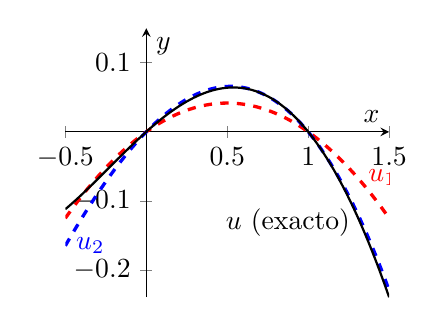
\begin{tikzpicture}
			\begin{axis}[domain=-.5:1.5, ymax=.15 ,samples=100, axis lines=middle, xlabel=$x$, ylabel=$y$, scale=.6]
				\addplot[color=red, very thick, dashed] {1/6*x*(1-x)} node[right, pos=.9]{$u_1$};
				\addplot[color=blue, very thick, dashed] {x*(1-x)*(7/29 + 5/116*x)} node[right, pos=0]{$u_2$};
				\addplot[color=black, thick] {1/(2*(1/e-1))*(1-e^(-x)) - 1/2*x^2 + x} node[left, pos=.9]{$u$ (exacto)};
			\end{axis}
		\end{tikzpicture}
		\caption{Comparación de la solución exacta con las aproximadas.}
		\label{fig:ed}
	\end{marginfigure}
\end{example}


\begin{example} \label{ex:galerkin2}
	\
	Otro ejemplo de aplicación del método de Galerkin: Resolver la barra de la fig. Adoptar $E = 1$.
	
	\begin{figure}[H]
		\centering
		\includestandalone[width=.8\textwidth]{figs/aproximados/corneta}
		\caption{Barra a tracción con sección variable.}
		\label{fig:ejm1}
	\end{figure}

\textit{Solución}:
\vspace{2mm}
		
	De la figura se obtienen las condiciones de frontera:
	\begin{equation*}
		\begin{cases}
			u(0) = 0 & \mbox{condición esencial} \\[2mm]
			\left. EA\dfrac{du}{dx} \right|_{x=180} = 100 & \mbox{condición natural}
		\end{cases}
	\end{equation*}
	
	\textbf{Solución exacta}
	
	La ecuación diferencial del problema es:
	\begin{equation*}
		\dfrac{d}{dx}\left( EA \dfrac{du}{dx} \right) + p = 0
	\end{equation*}
	
	en este caso $p = 0$, $E=1$.
	
	\[ A = \begin{cases}
		1 \, \unit{cm^2} & 0 \le x \le 100\\
		\left(1 + \dfrac{x-100}{40}\right)^2 \, \unit{cm^2} & 100 \le x \le 180
	\end{cases} \]
	
	La ED resulta:
	\[ \frac{d}{dx} \left(A \frac{du}{dx}\right) = 0 \]
	integrando y considerando la condición de frontera natural:
	\[A \frac{du}{dx} = cte. = 100\]
	volviendo a integrar:
	\[ u = \begin{cases}
		100x & 0 \le x \le 100\\
		2000\left(7 - \dfrac{80}{x - 60}\right) & 100 \le x \le 180
	\end{cases} \]
	
	
	\begin{equation*}
		\begin{split}
			\int_L \phi_i \dfrac{d}{dx}\left(EA\dfrac{du}{dx} \right)\, dx =& \underbrace{\int_{0}^{100} \phi_i \dfrac{d}{dx}\left( \dfrac{du}{dx} \right) \, dx}_{I_1} +\\ & \underbrace{\int_{100}^{180} \phi_i \dfrac{d}{dx}\left( A(x) \dfrac{du}{dx} \right) \, dx}_{I_2} = 0
		\end{split}
	\end{equation*}
	
	integrando por partes $I_1$ y observando que $\phi_i(0) = 0$ (debe cumplir las condiciones de frontera esenciales) se tiene:
	\begin{equation*}
		\begin{split}
			I_1 &= \left. \phi_i(100) \dfrac{du}{dx} \right|_{x=100} - \left.\phi_i(0) \dfrac{du}{dx} \right|_{x=0} - \int_{0}^{100} \dfrac{d \phi_i}{dx} \dfrac{du}{dx}\, dx \\[5mm]
			&= \left. \phi_i(100) \dfrac{du}{dx} \right|_{x=100} - \int_{0}^{100} \dfrac{d \phi_i}{dx} \dfrac{du}{dx} \, dx
		\end{split}
	\end{equation*}
	
	integrando por partes $I_2$:
	\begin{equation*}
		\begin{split}
			I_2 =& \left. \phi_i(180) A(180) \dfrac{du}{dx} \right|_{x=180} - \left. \phi_i(100) A(100) \dfrac{du}{dx} \right|_{x=100} \\ &- \int_{100}^{180} A(x) \dfrac{d \phi_i}{dx} \dfrac{du}{dx} \, dx
		\end{split}
	\end{equation*}
	
	Sumando $I_1 + I_2$, observando que $A(100) = 1$ y $A(180) \dfrac{du}{dx} |_{x=180} = 100$, se tiene
	\begin{equation}
		- \int_{0}^{100} \dfrac{d \phi_i}{dx} \dfrac{du}{dx}\, dx + 100 \phi_i(180) - \int_{100}^{180} A(x) \dfrac{d \phi_i}{dx} \dfrac{du}{dx}\, dx = 0
		\label{eq:g2}
	\end{equation}
	
	\begin{itemize}
		\item \textbf{Solución aproximada}
		\begin{equation}
			u(x) = a_0 + a_1 x + a_2 x^2
		\end{equation}
		Esta función debe satisfacer todas las condiciones de frontera.
		
		en donde se adoptan como funciones ponderadoras:
		\begin{equation}
			\begin{cases}
				\phi_1 = x \implies \dfrac{d \phi_1}{dx} = 1 \\[4mm]
				\phi_2 = x^2 \implies \dfrac{d \phi_2}{dx} = 2x
			\end{cases}
		\end{equation}
		
		en \eqref{eq:g2}
		\begin{equation}
			\systeme[a_1 a_2]{67a_1 + 17340a_2 = 2700, 867a_1 + 255568a_2 = 24300}
			\label{eq:sis1}
		\end{equation}
		
		de donde:
		\begin{equation}
			\begin{cases}
				a_1 = 128.6 \\ a_2 = -0.341
			\end{cases}
			\label{eq:coefs}
		\end{equation}
		
		por lo tanto la función aproximadora es:
		\begin{equation*}
			u_2(x) = 128.6x - 0.341 x^2
		\end{equation*}
		
		\item \textbf{Solución exacta}
		
		La solución exacta es:
		\begin{equation*}
			u(x) = \begin{cases}
				100 x & \mbox{en } 0 \le x \le 100 \\
				2000\left(7 - \dfrac{80}{x - 60}\right) & \mbox{en } 100 \le x \le 180
			\end{cases}
		\end{equation*}
	\end{itemize}
		
	Estos resultados se grafican en la fig. \ref{fig:compar}
	\begin{marginfigure}[-3cm]
		\centering
		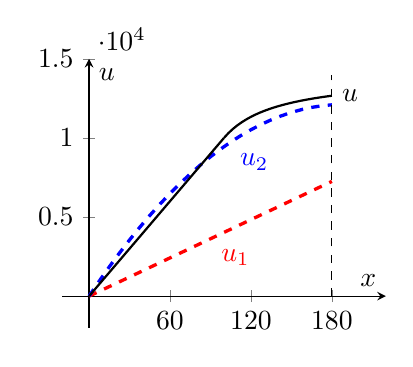
\begin{tikzpicture}
			\begin{axis}[scale=.6, domain=0:180, ymin=-2000, ymax=15000, xmin=-20, xmax=220, axis lines=middle, xlabel=$x$, ylabel=$u$, xtick={60, 120, 180}]
				\addplot[very thick, red, dashed] {2700/67*x} node[pos=.5, below right]{$u_1$};
				\vline{180};
				\addplot[very thick, blue, dashed] {67167900/522319*x - 178200/522319*x*x} node[pos=.8, below right]{$u_2$};
				\addplot +[mark=none, dashed, color=black] coordinates {(180, 0) (180, 14000)};
				\addplot[domain=0:100, thick, black] {100*x};
				\addplot[domain=100:180, thick, black] {14000 - 160000/(x - 60)} node[right]{$u$};
			\end{axis}
		\end{tikzpicture}
	\caption{Comparación de resultados}
	\label{fig:compar}
	\end{marginfigure}
	Los diagramas de:
	\begin{itemize}
		\item fuerza normal $N(x) = EA \dfrac{du}{dx}$;
		\item tensiones normales $\sigma(x) = E \dfrac{du}{dx}$, y
		\item deformaciones unitarias $\varepsilon(x) =  \dfrac{du}{dx}$,
	\end{itemize} para cada uno de los resultados obtenidos son:
	
	\begin{figure}[H]
		\centering
		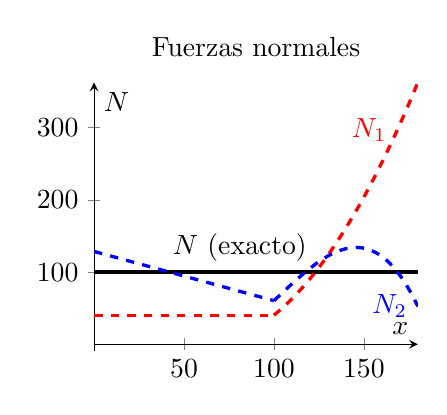
\begin{tikzpicture}
			\begin{axis}[scale=.6, domain=0:180, axis lines=middle, ymin=-10, xlabel=$x$, ylabel=$N$, title=Fuerzas normales]
				\addplot[very thick] {100} node[pos=.45, above]{$N$ (exacto)};
				\addplot[domain=0:100, red, very thick, dashed] {40.3};
				\addplot[domain=100:180, red, very thick, dashed] {(1 + (x-100)/40)^2*2700/67} node[pos=.8, left]{$N_1$};
				\addplot[domain=0:100, blue, very thick, dashed] {128.6 - 2*0.341*x};
				\addplot[domain=100:180, blue, very thick, dashed] {(1 + (x-100)/40)^2*(128.6 - 2*0.341*x)} node[left]{$N_2$};
			\end{axis}
		\end{tikzpicture}
	\end{figure}
		
	\begin{figure}[H]
		\centering
		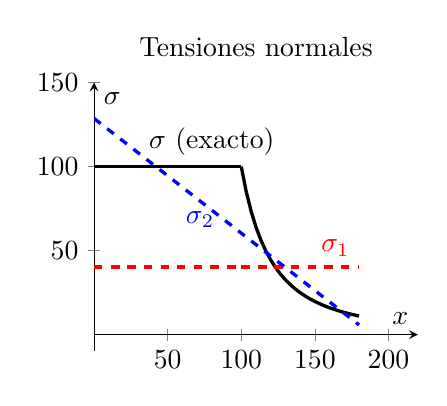
\begin{tikzpicture}
			\begin{axis}[scale=.6, domain=0:180, axis lines=middle, ymin=-10, ymax=150, xmax=220, xlabel=$x$, ylabel=$\sigma$, title=Tensiones normales]
				\addplot[very thick, domain=0:100] {100} node[pos=.8, above]{$\sigma$ (exacto)};
				\addplot[very thick, domain=100:180] {100/(1 + (x-100)/40)^2};
				\addplot[domain=0:100, red, very thick, dashed] {40.3};
				\addplot[domain=100:180, red, very thick, dashed] {2700/67} node[pos=.8, above]{$\sigma_1$};
				\addplot[blue, very thick, dashed] {128.6 - 2*0.341*x} node[pos=.4, below]{$\sigma_2$};
			\end{axis}
		\end{tikzpicture}
	\end{figure}
		
	\begin{figure}[H]
		\centering
		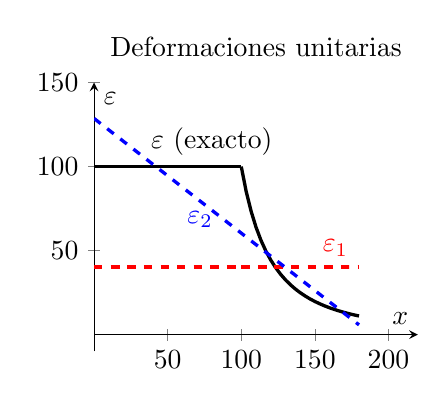
\begin{tikzpicture}
			\begin{axis}[scale=.6, domain=0:180, axis lines=middle, ymin=-10, ymax=150, xmax=220, xlabel=$x$, ylabel=$\varepsilon$, title=Deformaciones unitarias]
				\addplot[very thick, domain=0:100] {100} node[pos=.8, above]{$\varepsilon$ (exacto)};
				\addplot[very thick, domain=100:180] {100/(1 + (x-100)/40)^2};
				\addplot[domain=0:100, red, very thick, dashed] {40.3};
				\addplot[domain=100:180, red, very thick, dashed] {2700/67} node[pos=.8, above]{$\varepsilon_1$};
				\addplot[blue, very thick, dashed] {128.6 - 2*0.341*x} node[pos=.4, below]{$\varepsilon_2$};
			\end{axis}
		\end{tikzpicture}
	\end{figure}
\end{example}

\section{Trabajo virtual}

Aplicando el método de Galerkin a la ecuación diferencial \eqref{eq:equil} $\nabla \bm{\sigma} + \mathbf{f} = 0$, suponiendo que las función vectorial de peso es $\bm{\phi}(\mathbf{r})$, se tiene:

\begin{equation}
	\int_V \bm{\phi}^T \left( \nabla \bm{\sigma} + \mathbf{f} \right) \, dV = \int_V \bm{\phi}^T \nabla \bm{\sigma} \, dV + \int_V \bm{\phi}^T \mathbf{f}\, dV = 0
	\label{eq:tv1}
\end{equation}

Observe que:
\begin{equation}
	\nabla \left( \bm{\phi}^T \bm{\sigma} \right) = \left(\nabla \bm{\phi}^T\right) \colon \bm{\sigma} + \bm{\phi}^T \nabla \bm{\sigma}
	\label{eq:tv2}
\end{equation}
entonces:
\begin{equation}
	\int_V \left(\nabla \bm{\phi}^T\right) \colon \bm{\sigma}\, dV = \int_V \nabla \left( \bm{\phi}^T \bm{\sigma} \right) \, dV - \int_V \bm{\phi}^T \nabla \bm{\sigma} \, dV
	\label{eq:tv3}
\end{equation}

por el teorema de Gauss y \eqref{eq:tSigma}:
\begin{equation}
	\int_V \nabla \left( \bm{\phi}^T \bm{\sigma} \right) \, dV = \int_S \bm{\phi}^T \bm{\sigma} \mathbf{n}\, dS = \int_S \bm{\phi}^T \mathbf{T} \, dS
	\label{eq:tv4}
\end{equation}

De \eqref{eq:tv1} y \eqref{eq:tv4} en \eqref{eq:tv3}
\begin{equation}
	\int_V \left(\nabla \bm{\phi}^T\right) \colon \bm{\sigma}\, dV = \int_V \bm{\phi}^T \mathbf{f}\, dV + \int_S \bm{\phi}^T \mathbf{T} \, dS
	\label{eq:tv5}
\end{equation}

agregando el trabajo virtual de las cargas puntuales, se tiene el teorema del trabajo virtual, que expresa que \textit{el trabajo virtual interno es igual al trabajo virtual externo}:
\begin{equation}
	\boxed{\int_V \underline{\bm{\varepsilon}}^T_{(\phi)} \underline{\bm{\sigma}} \, dV = \int_V \bm{\phi}^T \mathbf{f}\, dV + \int_S \bm{\phi}^T \mathbf{T} \, dS + \sum_i \bm{\phi}^T_i \mathbf{P}_i}
	\label{eq:tv6}
\end{equation}


\subsection{Caso unidimensional}

Para una dimensión, la ec. \eqref{eq:tv6} se convierte en:
\begin{equation}
	\int_L N \dfrac{d \phi}{dx} \, dx = \int_L \phi p \, dx + \sum_i \phi_{(i)} P_i
\end{equation}

En donde $N$ es la fuerza normal, $p$ la carga por unidad de longitud y $P_i$ cargas puntuales.

Además, $N = EA \dfrac{du}{dx}$, con $E$: módulo de Young y $A$: área de la sección transversal, la ecuación anterior se transforma en la siguiente:
\begin{equation}
	\boxed{\int_L EA \dfrac{du}{dx} \dfrac{d \phi}{dx} dx = \int_L \phi p \, dx + \sum_i \phi_{(i)} P_i}
	\label{eq:GUni}
\end{equation}

Una \textbf{deducción alternativa} de \eqref{eq:GUni}, se muestra a continuación:

La ecuación diferencial del caso unidimensional es:
\begin{equation}
	\dfrac{d}{dx} \left( EA \dfrac{du}{dx} \right) + p = 0
\end{equation}

ahora, se multiplica por la función de peso $\phi(x)$ e integra en toda la longitud de la barra:
\begin{equation}
	\int_L \phi \left[ \dfrac{d}{dx} \left( EA \dfrac{du}{dx} \right) + p \right] \, dx = 0
\end{equation}

de donde:
\begin{equation}
	\int_L \phi \dfrac{d}{dx} \left( EA \dfrac{du}{dx} \right) \, dx = -\int_L \phi p \, dx
	\label{eq:g1}
\end{equation}

integrando por partes el miembro izquierdo:
\begin{equation}
	\begin{split}
		\int_L \phi \dfrac{d}{dx} \left( EA \dfrac{du}{dx} \right) \, dx &= \phi EA \dfrac{du}{dx} \Big ]_{x=0}^{x=L} - \int_L EA \dfrac{du}{dx} \dfrac{d \phi}{dx} \\ & = \phi(L)P(L) - \phi(0)P(0) - \int_L EA \dfrac{du}{dx} \dfrac{d \phi}{dx}
	\end{split}
	\label{eq:partes}
\end{equation}

En donde $P(0)$ y $P(L)$ son las cargas puntuales en los extremos.

Finalmente, reuniendo \eqref{eq:g1} y \eqref{eq:partes}, se obtiene \eqref{eq:GUni}.
\begin{example}
	Utilizando el método del trabajo virtual, resolver nuevamente la barra de la figura \ref{fig:ejm1}, la cual se copia aquí. Adoptar $E=1$.
	
	\begin{figure}[H]
		\centering
		\includestandalone[width=.7\textwidth]{figs/aproximados/corneta}
		\repeatcaption{fig:ejm1}{Barra a tracción}
	\end{figure}
	
\textbf{Solución}

		Se aplicará la ec. \eqref{eq:GUni} del método de trabajo virtual:
		
		\begin{equation*}
			\int_L EA \dfrac{du}{dx} \dfrac{d \phi}{dx} dx = \int_L \phi p \, dx + \sum_i \phi_{(i)} P_i
		\end{equation*}
		
		\begin{itemize}
			\item \textbf{Primera aproximación}:
			
			Se toma como función aproximadora $u = ax$ y como desplazamiento virtual $\phi = x$, las cuales cumplen con las \acrlong{cfe}, entonces:
			
			\begin{equation}
				\begin{cases}
					u = a x \implies \dfrac{du}{dx} = a\\[4mm]
					\phi = x \implies \dfrac{d \phi}{dx} = 1
				\end{cases}
			\end{equation}
			
			observando que $p=0$, se realizan los cálculos de la ecuación \eqref{eq:GUni}:
			
			\begin{equation}
				\int_{0}^{100} a \, dx + \int_{100}^{180} a\left[1 + \dfrac{\left(x-100\right)}{40}\right]\, dx = 18000
			\end{equation}
			
			de donde:
			
			\begin{equation}
				a = \dfrac{2700}{67}
			\end{equation}
			
			como en \eqref{eq:a1}.
			
			\item \textbf{Segunda aproximación}
			
			Para lograr una función aproximadora cuadrática de la forma $u(x) = a_1x + a_2x^2$, debemos considerar dos campos de desplazamientos virtuales, se adoptan:
			
			\begin{equation}
				\begin{cases}
					\phi_1 = x \implies \dfrac{d \phi_1}{dx} = 1\\[4mm]
					\phi_2 = x^2 \implies \dfrac{d \phi_2}{dx} = 2x
				\end{cases}
			\end{equation}
			
			para cada uno de los los cuales \eqref{eq:GUni} pasa a ser:
			\begin{equation}
				\footnotesize
				\begin{split}
					& \int_{0}^{100} \left(a_1 + 2a_2x \right) \, dx + \int_{100}^{180} \left[1 + \dfrac{ \left( x-100 \right)}{40} \right] \left(a_1 + 2a_2x \right) \, dx \\[4mm]&= 18000 \\[4mm]
					& \int_{0}^{100} 2ax \left(a_1 + 2a_2x \right) \, dx + \int_{100}^{180} 2x \left[1 + \dfrac{ \left( x-100 \right)}{40} \right] \left(a_1 + 2a_2x \right) \, dx \\[4mm]&= \num{3240000}
				\end{split}
				\label{eq:int1}
			\end{equation}
			
			realizando las integrales se obtiene el siguiente sistema de ecuaciones lineales:
			
			\begin{equation}
				\systeme[a_1 a_2]{67a_1 + 17340a_2 = 2700, 867a_1 + 255568a_2 = 24300}
			\end{equation}
			
			que es idéntico a \eqref{eq:sis1}, ejm. \ref{ex:galerkin2}, como era de esperarse ya que, en realidad, las integrales \eqref{eq:int1} son idénticas a \eqref{eq:g2} del ejm. \ref{ex:galerkin2}.
		\end{itemize}
\end{example}

\subsection{Trabajo virtual en vigas}
Para el caso de vigas con cargas distribuidas $q$, la ec. \eqref{eq:tv6} se convierte en:

\begin{equation}
	\int_L EI \frac{d^2\phi}{dx^2} \frac{d^2v}{dx^2} \, dx = \int_L \phi q \, dx + 
	\sum_i \phi_{(i)} P_i
	\label{eq:tv-vigas}
\end{equation}

\section{Ejercicios resueltos}

\subsection{Vigas}

\begin{example} \label{ex:viga0}
	
	Para la viga y la carga que se muestra en la fig. \ref{fig:viga0}, determinar el 
	campo de desplazamientos por los métodos de Rayleigh-Ritz y Galerkin. Suponer $EI = 1$.
	
\begin{marginfigure}[-.5cm]
	\centering
	\includestandalone[width=\textwidth]{figs/aproximados/viga0}
	\caption{Viga con carga variable}
	\label{fig:viga0}
\end{marginfigure}

\textbf{Solución}

De acuerdo al grado del polinomio de la carga distribuida, la deformada será de grado 5.
\[ v(x) = a_0 + a_1x + a_2 x^2 + a_3 x^3 + a_4 x^4 + a_5 x^5\]

Se observa que las condiciones esenciales (o cinemáticas) de frontera son:
\[ v(0) = 0; \qquad v'(0)=0; \qquad v(1) = 0 \]
por lo tanto:
\[ a_0 = 0; \qquad a_1 = 0; \qquad a_2 = -a_{3} - a_{4} - a_{5} \]

y la función aproximadora se reduce a:
\begin{equation}
	v(x) = - \left(a_{3} + a_{4} + a_{5}\right) x^{2} + a_{3} x^{3} + a_{4} x^{4} + a_{5} x^{5} 
	\label{eq:v0}
\end{equation}

La condición natural (o estática) de frontera es:

\begin{equation}
	\left. EI \frac{d^2v}{dx^2} \right|_{x=1} = 0
\end{equation}

\begin{itemize}
	\item \textbf{Método de Rayleigh-Ritz}
	
	La ecuación de la energía potencial, conforme a \eqref{eq:energia-vigas}, es:
	\[ \Pi = \frac{1}{2} \int_L EI \left( \frac{d^2v}{dx^2} \right) \, dx - \int_L v q \, dx \]
	
	La primera y segunda derivadas de \eqref{eq:v0} son:
	\[ v'(x) = -2 \left(a_{3} + a_{4} + a_{5}\right) x + 3 a_{3} x^{2} + 4 a_{4} x^{3} + 5 a_{5} x^{4} \]
	\[ v''(x) = -2 \left(a_{3} + a_{4} + a_{5}\right) + 6 a_{3} x + 12 a_{4} x^{2} + 20 a_{5} x^{3} \]
	
	según dato del problema \[ q = 1 - x \]
	sin embargo, para ser coherentes con las demás convenciones de signo, al apuntar la
	función $q$ hacia abajo debemos tomar:

	\[q = x - 1\]
	
	Llevando estas ecuaciones en la expresión de la energía potencial e integrando se obtiene:
	\[ \Pi = 2 a_{3}^{2} + 8 a_{3} a_{4} + 12 a_{3} a_{5} + \frac{a_{3}}{30} + \frac{42 a_{4}^{2}}{5} + 26 a_{4} a_{5} + \frac{a_{4}}{20} + \frac{144 a_{5}^{2}}{7} + \frac{5 a_{5}}{84}\]
	
	Las derivadas parciales de $\Pi$ respecto de $a_2$, $a_3$ y $a_4$ llevan al siguiente sistema de ecuaciones:
	
	\[\systeme{4 a_{3} + 8 a_{4} + 12 a_{5} = \frac{1}{30}, 
	8 a_{3} + \frac{84}{5} a_{4} + 26 a_{5} = \frac{1}{20},
	12 a_{3} + 26 a_{4} + \frac{288}{7}a_{5} = \frac{5}{84}}
	\]
	cuya solución es:
	\[ a_3 = \frac{1}{15}; \quad a_4 = -\frac{1}{24}; \quad a_5 = \frac{1}{120} \]
	
	La función aproximadora es en consecuencia:
	\[ v(x) = -\frac{1}{30}x^2 + \frac{1}{15}x^3 - \frac{1}{24}x^4 + \frac{1}{120}x^5 \]
	
	\item \textbf{Método de Galerkin}
	
	La ecuación diferencial de campo es:

	\[ \frac{d^2}{dx^2} \left( EI \frac{d^2v}{dx^2} \right) - q = 0 \]


	Debemos expresar la función aproximadora como combinación lineal de funciones $\phi_i$.
	
	Reordenando la expresión de $v(x)$ dada en \eqref{eq:v0}, se obtiene:
	\[ \begin{split}
		v(x) &= x^{2} \left(x - 1\right) \left(a_{3} + a_{4} \left(x + 1\right) + a_{5} \left(x^{2} + x + 1\right)\right) \\
		&= a_3\phi_1 + a_4\phi_2 + a_5 \phi_3
	\end{split} \]
	siendo:
	\[ \phi_1 = x^2(x-1); \quad \phi_2 = x^2 (x^2 -1); \quad \phi_3 = x^2(x^3-1) \]
	notar que todas las $\phi_i$ cumplen con las condiciones esenciales de frontera:
	\[ \phi_i(0) = 0; \quad \phi_i(1) = 0; \quad \phi_i'(0) = 0 \]
	
	La ecuación de campo, en este caso, es:
	\[ \frac{d^4v}{dx^4} - q = 0 \]
	en donde se ha considerado $q$ positivo hacia arriba.
	
	El error debe ser ortogonal a las funciones $\phi_i$, entonces:
	\[ \int_L \left( \frac{d^4v}{dx^4} - q \right) \phi_i dx = 0\]
	
	\[ \int_L \frac{d^4v}{dx^4} \phi_i dx = \int_L q \phi_i dx  \]
	integrando por partes, dos veces, el miembro izquierdo:
	\[ \begin{split}
		\int_L \frac{d^4v}{dx^4} \phi_i dx &= \left[ \frac{d^3v}{dx^3} \phi_i \right]_0^1 - 
	\int_L \frac{d^3v}{dx^3} \frac{d\phi_i}{dx} dx = - \int_L \frac{d^3v}{dx^3} \frac{d\phi_i}{dx} dx \\
	&= -\left[\frac{d^2v}{dx^2} \frac{d\phi_i}{dx}\right]_0^1 + \int_L \frac{d^2v}{dx^2} 
	\frac{d^2\phi_i}{dx^2}\\
	&= -v''(1) \phi'(1) + \int_L \frac{d^2v}{dx^2} \frac{d^2\phi_i}{dx^2}dx
	\end{split} \]

	En donde se han considerando las condiciones de frontera esenciales, si además
	se considera la condición de frontera natural, se llega a la expresión:
	\[ \int_L \frac{d^2v}{dx^2} \frac{d^2\phi_i}{dx^2}dx = \int_L q \phi_i dx \]

	Esta es, precisamente, la expresión del trabajo virtual tal como se deduciría de la
	ec. \eqref{eq:tv-vigas}.

	El cálculo de las integrales indicadas, para cada función $\phi_i$ lleva al siguiente
	sistema de ecuaciones:

	\[ \systeme{2a_4 + 6a_5 = -\frac{1}{30},
	\frac{16}{5}a_{4} + 10 a_{5} = - \frac{1}{20},
	4 a_{4} + \frac{90}{7}a_{5} = -\frac{5}{84}}\]

	El sistema es consistente y tiene las soluciones:

	\[ a_4 = -\frac{1}{24}; \quad a_5 = \frac{1}{120} \]

	Como el sistema resultó ser independiente de $a_3$, para hallarlo, se utiliza la condición de 
	frontera natural con los valores hallados de $a_4$ y $a_5$, de donde resulta:
	\[a_3 = \frac{1}{15} \]

	Se llega por tanto a la misma función aproximadora obtenida con el método de 
	Rayleigh-Ritz.
	
\end{itemize}
	
\end{example}